\section{Introduction} 
\label{sec:intro}

%% Why soft robots?
%% Body softness has been shown to be useful for robots operating in unstructured/unpredictable environments, or alongside humans, but hard to control.
Soft robots have bodies made out of intrinsically soft and/or compliant materials.
This inherent softness enables them to safely interact with delicate objects, and to passively adapt their shape to unstructured environments \cite{rus2015design}.
Such traits are desirable for robotic applications that demand safe human-robot interaction such as wearable robots, in-home assistive robots, and medical robots.
Unfortunately, the soft bodies of these robots also impose modeling and control challenges, which have restricted their functionality to date. 
In fact, many novel soft devices such as soft grippers (cite), crawlers (cite), and swimmers (cite) exploit the flexibility of their bodies to achieve coarse behaviors such as grasping and locomotion, but do not exhibit precise control capabilities \Dan{don't forget to add citations here}.
% Emulating the functionality of the dexterous and precise soft systems found in nature such as octopus arms, elephant trunks, and tongues stems from the inherent difficulty of modeling continuum structures and controlling nonlinear dynamical systems.

% Unfortunately, their soft bodies also make soft robots notoriously difficult to model and control, limiting their functionality to date. 
% While their compliance enables such behavior it also makes soft robots challenging to model and control \cite{rus2015design}.

% Soft systems found in nature such as octopus arms, elephant trunks, and tongues display incredible dexterity and precision \cite{vogel2000cats}, but such functionality has yet to be realized in soft robots.
% Many novel devices such as soft grippers (cite), crawlers (cite), and swimmers (cite) exploit the flexibility of their bodies to achieve coarse behaviors such as grasping and locomotion, but do not exhibit precise control capabilities
% can be attributed to two innate characteristics of soft systems: continuum structure, and nonlinear dynamical behavior. 


%% Technical challenges to modeling: continuum structure
% Even building models for soft robots presents a challenge.
The challenge in constructing such precise control techniques is due in large part to the difficulty of devising models of soft robots that are amenable to model based control design techniques.
% Mathematical models are a convenient tool for predicting behavior and designing controllers for robots, but useful models are not as readily available for soft robots as for rigid-bodied ones \Ram{citation?}.
Consider for instance rigid-bodied robotic systems that are made up of rigid links connected together by discrete joints.
% Rigid-bodied robots consist of rigid links connected together by discrete joints.
%It has been shown that the full geometry of a rigid-bodied system can be described in terms of joint deformations, making joint deformations the canonical choice of state variables for rigid-bodied robots \cite{spong2008robot}.  %[Brent thinks the following would be a little easier to read:]
Since joint displacements can be used to fully describe the configuration of a rigid-bodied system, joint displacements and their derivatives make a natural choice for the state variables for rigid-bodied robots \cite{spong2008robot}.
One can use this choice of state variables to describe the dynamics of the rigid-bodied robot.
This, as a result, makes the application of model-based control design techniques such as feedback linearization \cite{}, nonlinear model predictive control \cite{}, LQR-trees \cite{}, sequential action control \cite{ansari2016sequential}, and others feasible. \Dan{don't forget to add citations here} 

Soft robots, in contrast, do not exhibit localized deformation at discrete joints, but instead deform continuously along their bodies and have infinite degrees-of-freedom.
In the absence of joints, there does not yet exist a canonical choice of state variables to describe the geometry of a soft robot.
% Instead, it is common practice to choose a state made up of observable parameters, such as end-effector position (cite our koopman paper), curvature of body (cite), or fluid pressure (cite) \Dan{think of better example(s)}.
As a result, existing representations are typically only rich enough to describe the system under restrictive simplifying assumptions.
For example, the popular piecewise constant curvature model \cite{webster2010design} provides a low-dimensional description of the shape of continuum robots, but only under the assumption that bending occurs in sections of constant curvature.
Other simplified models such as pseudo-rigid-body (cite) and quasi-static \cite{bruder2018iros} (cite others), have demonstrated sufficient accuracy for some objectives (cite), \Dan{don't forget to add citations here} 
but they are only able to describe the behavior in a subset of configurations of the soft robot which can make applying model-based control design techniques impractical. 

%% FIGURE: Overview of the different system representations and control approaches
\begin{figure}
    \centering
    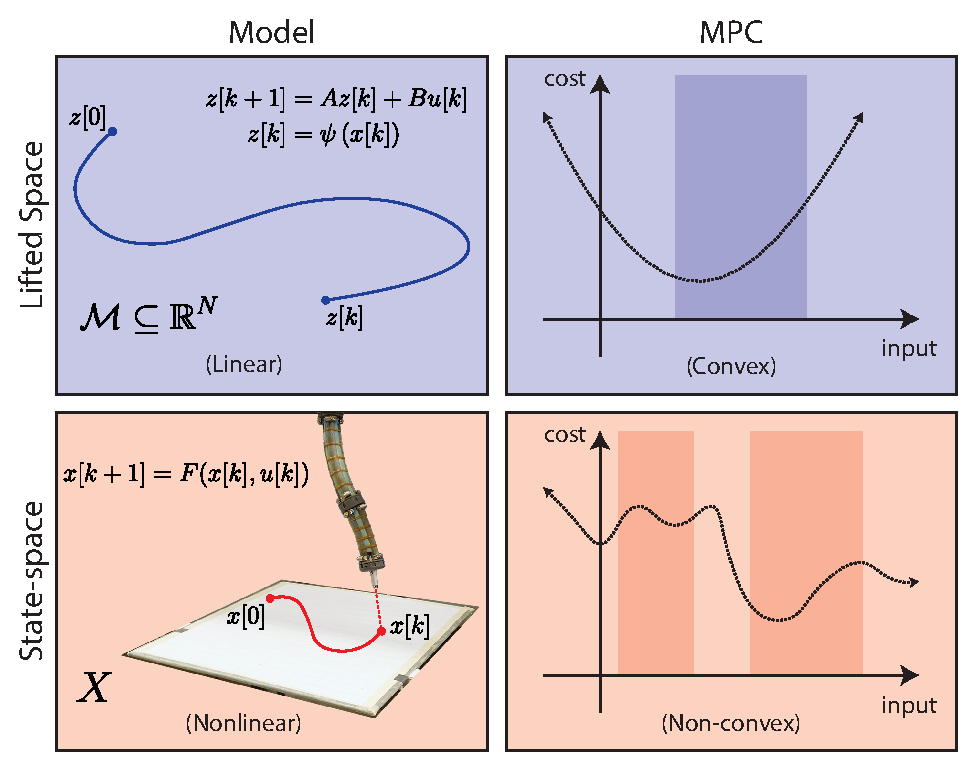
\includegraphics[width=\linewidth]{figures/overview_v8.pdf}
    \caption{A nonlinear dynamical system (bottom-left) has a \emph{linear} representation in the \emph{lifted} space made up of all real-valued functions (top-left). While a model predictive controller (MPC) designed for the nonlinear system in state-space requires solving a non-convex optimization problem to choose inputs at each time-step (bottom-right), this problem is convex for an MPC controller designed for the lifted linear system (top-right). This paper develops a data driven method to construct such a lifted model representation  for soft robotic systems in the presence of outliers and a convex, model-based control design technique for such systems. }
    \vspace*{-0.5cm}
    \label{fig:overview}
\end{figure}

%% data-driven models: don't make assumptions but not great for building controllers
% \Dan{This paragraph is a mess. Going to step away and come back to it}
Alternatively, data-driven methods, such as machine learning and neural networks, can be applied to construct models for soft robots without making structural simplifying assumptions.
Such models serve as a ``black-box'' by mapping from inputs to outputs and have been shown to predict behavior well across various configurations of the soft robot  \cite{gillespie2018learning, thuruthel2018model}.
However, since no explicit model is constructed, it can be challenging to apply existing model-based control design techniques.
% While such ``black-box'' models have been shown to predict behavior well, they offer little insight when it comes to controller design.
% \Ram{can you be more explicit here?} 

%% Technical challenge to control: Nonlinear dynamical behavior (think about this more and fix it)
% The inherently nonlinear dynamical behavior of soft robots presents a control challenge (CITE LASCHI CONTROL PAPER).
% Linear dynamical systems obey the \emph{superposition principle} (cite), which has enabled the development of powerful tools that render the task of controlling linear systems almost trivial.
% Unfortunately, the superposition principle does not hold for nonlinear dynamical systems and consequently there is no universal approach to controlling them.
% Numerical control techniques, such as nonlinear model predictive control (NMPC), have become popular due to ongoing increases in computational power and affordability.
% However, such methods require iteratively solving nonlinear non-convex optimization problems, for which global convergence is not guaranteed \cite{boyd2004convex}.
% which suffer from numerical issues such as suboptimal convergence and slow execution . 
% Numerical solvers may converge to suboptimal local extrema rather than optimal values.
% they are also slow...
% While this problem is not limited to soft robots (few mechanical systems exhibit completely linear dynamic behavior), soft robots are not as amenable to approximate linear descriptions as many other systems.

%% Koopman approach exists and can help here, it just needs some tweaks to work well for a real system
Koopman Operator Theory offers an approach that can overcome the challenges of modeling and controlling soft robots.
The Koopman operator approach is data-driven yet produces an explicit control-oriented model that is linear (though higher dimensional).
% Laid out in \citet{korda2018linear}, 
The approach leverages the linear structure of the Koopman operator to construct linear models of nonlinear controlled dynamical systems from input-output data \cite{bruder2018nonlinear, mauroy2016linear}, and to control them using established linear control methods \cite{Abraham-RSS-17, korda2018linear}.
In theory, this approach involves \emph{lifting} the state-space to an infinite-dimensional space of scalar functions (referred to as observables), where the flow of such observables along trajectories of the nonlinear dynamical system is described by the \emph{linear} Koopman operator.
In practice, however, it is not feasible to compute an infinite-dimensional operator, so a modified version of the Extended Dynamic Mode Decompostion (EDMD) is employed to compute a finite-dimensional projection of the Koopman operator onto a finite-dimensional subspace of all observables (scalar functions).
This approximation of the Koopman operator describes the evolution of the values of the output variables themselves, provided that they lie within the finite subspace of observables upon which the operator is projected.
Hence, this approach makes it possible to control the output of a nonlinear dynamical system using a linear controller designed for its linear Koopman representation.

%% Why this approach is uniquely well suited for soft robots: 
The Koopman approach to modeling and control is well suited for soft robots for several reasons.
Soft robots pose less of a physical threat to themselves or their surroundings when subjected to random control inputs than conventional rigid-bodied robots. 
This makes it possible to safely collect input-output data over a wide range of operating conditions, and to do so in an automated fashion. 
Furthermore, since the Koopman procedure is entirely data-driven, it inherently captures input-output behavior and avoids the ambiguity involved in choosing a discrete set of states for a structure with infinite degrees of freedom.
% Soft robots are also nonlinear dynamical systems, but this approach generates a linear system representation.
% As will be shown later, this linear representation can be used to construct a controller which computes control inputs by solving a convex optimization problem at each time step.

%% Our contribution: Modifications/additions needed to get this to reliably work for a real system
% This work applies the Koopman based system identification method from \citet{mauroy2016linear} and the Koopman based model predictive control method from \citet{korda2018linear} to a real soft robotic system.
The work presented here can be considered an extension of the work on Koopman-based modeling and control of \citet{mauroy2016linear} and \citet{korda2018linear}.
The novel contributions of this work, as depicted in Fig. \ref{fig:overview} are:
\begin{enumerate}
    \item An extension to the Koopman system identification procedure described in \cite{mauroy2016linear} to make the resulting Koopman operator both more sparse and less sensitive to outliers and noise in the training data,
    \item The application of this identified Koopman model for model predictive control of a physical soft robotic system.
\end{enumerate}
% We achieve (1) by introducing an $L^1$ penalty term into the least-squares optimization problem used to solve for the approximate Koopman operator.
Contribution (1) arose by necessity from the pursuit of contribution (2), since real mechanical systems suffer from both noise and computational limitations. \Dan{Rewrite this last sentence.} \Ram{my suggestion is that you highlight in the previous paragraph (the one about the utility of applying Koopman operator theory to soft robots) that pressure regulators for soft robots suck so they are super noisy which can make identifying such a Koopman model in practice difficult.}
% Data collected from physical mechanical systems is prone to noise, which can lead to over-fitting of data-driven models.
% Because real mechanical systems suffer from noise this step is 
% Both of these are desirable features when working with real systems, which suffer from noise and computational limitations.



%% Outline
The rest of this paper is organized as follows:
In Section \ref{sec:sysid} we formally introduce the Koopman operator and describe how it is used to construct linear models of nonlinear dynamical systems. 
In Section \ref{sec:mpc} we describe how the Koopman model can be used to construct a linear model predictive controller.
In Section \ref{sec:experiments} we describe the soft robot and the set of experiments used to evaluate the performance of a Koopman-based MPC controller.
In Section \ref{sec:conclusion} concluding remarks and perspectives are provided.





% %% Solution: Data-driven/linear representation, description of koopman approach
% In this paper, we present a novel method for the modeling and control of soft robots based on Koopman Operator Theory.
% This method addresses the challenges of modeling and control by offering a way to build a \emph{linear} model from data that still captures the \emph{nonlinear} input-output behavior of a soft robot.
% This approach is based on the system identification method originally presented in \citet{mauroy2017koopman} and the control approach laid out in \citet{korda2018linear}.